%% Zweiseitiges Layout
\documentclass[11pt,twoside,a4paper,fleqn]{report}
\usepackage[top=3cm, bottom=2.5cm, left=4cm, right=3cm]{geometry}

%% Schriftbild
\usepackage{lmodern}  % Latin Modern Zeichensatz
\usepackage[utf8]{inputenc}  % Unterstützung von Umlauten im Quelltext
\usepackage[T1]{fontenc}  % Korrekte Umlaute im PDF
\usepackage[english]{babel}  % Silbentrennung nach neuer Rechtschreibung
\renewcommand{\familydefault}{\sfdefault}  % Serifenlose Schrift
\usepackage{setspace}\onehalfspacing  % 1.5-facher Zeilenabstand
\renewcommand{\arraystretch}{1.5}  % 1.5-facher Zeilenabstand (Tabellen)
\setlength{\parindent}{0pt}  % Keine Einrückung am Beginn von Absätzen
\usepackage{emptypage}
\usepackage{placeins} % plaziert figures in die richtige section
\usepackage{multirow}
\sloppy  % Weniger Silbentrennung

% Kopfzeile: Section auf linker Seite, Subsection auf rechter Seite
\usepackage{fancyhdr}
\pagestyle{fancy}
\renewcommand{\chaptermark}[1]{\markboth{#1}{}}
\renewcommand{\sectionmark}[1]{\markright{\thesection\ #1}}
\fancyhf{}
\fancyhead[LE,RO]{\small{\thepage}}
\fancyhead[LO]{\small{\rightmark}}
\fancyhead[RE]{\small{\leftmark}}
\renewcommand{\headrulewidth}{0.5pt}
\renewcommand{\footrulewidth}{0pt}
\fancypagestyle{plain}{%
  \fancyhead{}
  \renewcommand{\headrulewidth}{0pt}
}
%% Drawing:

\usepackage{tikz}
\usepackage{pgfplots}
\usetikzlibrary{math} %needed tikz library
\pgfplotsset{compat=1.11}
\usetikzlibrary{calc}
%\pgfmathdeclarefunction{gauss}{3}{%
%  \pgfmathparse{1/(sqrt(pow(#2,2)*2*pi))*exp(-(pow((#3-#1),2))/(2*pow(#2,2)))}%
%}
\pgfmathdeclarefunction{gauss}{4}{%A,mu,sigma,x
	\pgfmathparse{#1*(exp(-(pow((#4-#2),2))/(2*pow(#3,2))))}%
}
\pgfmathdeclarefunction{invgauss}{2}{%
	\pgfmathparse{sqrt(-2*ln(#1))*cos(deg(2*pi*#2))}%
}
\pgfmathsetseed{12344}%

%% Literaturverzeichnis (BibTex)
\usepackage{natbib}
\bibliographystyle{apalike}  % Layout des Literaturverzeichnisses

%% Verlinkung von Inhaltsverzeichnis, Bildern und Formeln
\usepackage[pagebackref]{hyperref}  % Verlinkung von URLs und Referenzen
\usepackage{color}  % Definition der Linkfarben
\definecolor{DarkRed}{rgb}{0.5,0,0}
\definecolor{Black}{rgb}{0,0,0}
\hypersetup{
  colorlinks,
  citecolor=Black,
  linkcolor=Black,
  urlcolor=Black}

%% Mathematikumgebung
\usepackage{mathtools}
\usepackage{amsmath}
\usepackage{amssymb}  % Erweiterte Bibliothek mathematischer Symbole
%\usepackage{euler}  % Serifenlose Schrift in Formelumgebungen
\usepackage[makeroom]{cancel}  % Durchstreichen von Termen
\renewcommand{\deg}{\ensuremath{^{\circ}}}  % Grad Zeichen im Text
\renewcommand{\epsilon}{\varepsilon}  % Nutze richtiges Epsilon

%% Grafikumgebungen
\usepackage{graphicx}  % Erweiterte Grafikumgebung
\usepackage{float}  % Automatische Positionierung von Bildern
\usepackage{subcaption}  %  Bildunterschriften für subfigures

%% Formeln, Bilder und Tabellen pro section nummerieren
\numberwithin{equation}{chapter}
\numberwithin{figure}{chapter}
\numberwithin{table}{chapter}

%% Listenumgebung
\usepackage{enumerate}
\usepackage{textcomp}  % Korrekte serifenlose Aufzählungszeichen

%% Farbige Umrahmungen
\usepackage{framed}
\definecolor{shadecolor}{rgb}{0.9,0.9,0.9}

%% Blindtext zum Testen des Layouts
\usepackage{blindtext}

%% Inhalt der Titelseite


%%%%%%%%%%%%%%%%%%%%%%%%%%%%%%%%%%%%%%%%%%%%%%%%%%%%%%%%%%%%%%%%%%%%%%
\setcounter{section}{0}
\begin{document}
	\thispagestyle{empty}
	\begin{center}
		\hspace*{0pt}\vfill
		\begin{Huge}
			Probabilistic Radar-Based Precipitation Nowcasting
		\end{Huge}
		\vfill
		\begin{minipage}{0.5\textwidth}
			\centering
			%\begin{flushleft}
				\begin{large}
					Masterthesis by
				\end{large}
				\\\vspace{0.5cm}
				\begin{huge}
					Simon Michel
				\end{huge}
			%\end{flushleft}
		\end{minipage}
		\vfill
		
		\begin{minipage}{0.5\textwidth}
			\centering
			%\begin{flushleft}
				\begin{large}
					%Matrikelnummer: 6353359\\
					Universität Hamburg\\
					Fachbereich Geowissenschaften
				\end{large}
			%\end{flushleft}
		\end{minipage}
		\vfill
		
		\begin{minipage}{0.5\textwidth}
			\centering
			%\begin{flushleft}
				\begin{large}
					%Matrikelnummer: 6353359\\
					Erstgutachter: Dr. Marco Clemens\\
					Zweitgutachter: Prof. Dr. Felix Ament
				\end{large}
			%\end{flushleft}
		\end{minipage}
		\vfill
		\begin{minipage}{0.5\textwidth}
			\centering
			%\begin{flushleft}
				\begin{large}
					Hamburg, \today
				\end{large}
			%\end{flushleft}
		\end{minipage}
		\vfill
	\end{center}
	
	\newpage
	\thispagestyle{empty}
	\null
	\vfill
	Masterthesis im Fachbereich Geowissenschaften der Universität Hamburg\\
	Thema der Arbeit: \glqq Probabilistic Radar-Based Precipitation Nowcasting\grqq
	
	
\newpage
\renewcommand{\abstractname}{\huge \flushleft Abstract}
\begin{abstract}
\null
\end{abstract}
\thispagestyle{empty}
\pagestyle{empty}
\tableofcontents
\listoffigures
\listoftables
\newpage\pagestyle{fancy}
\chapter{Introduction}
\pagenumbering{arabic}
\chapter{Data}
\section{DWD Radar Data}
Boostedt DWD radar site: 54.0055° N, 10.04683° E, 124.6 m height

Precipitation scan: 0.5° ,following orographie (150 km range)
250m range gates, 1° azimuth steps
5 minute time resolution
C-Band
100 km x 100 km box around PATTERN radar position taken from the whole radar image
\section{PATTERN Radar Data}
% https://wetterradar.uni-hamburg.de/index.php?id=4035
PATTERN Hamburg radar position: 53.56833°N, 9.97997° E, ~80m height

60m range gates, 1° azimuth steps (20 km range)
30s time resolution
X-Band

\begin{figure}
	\centering
	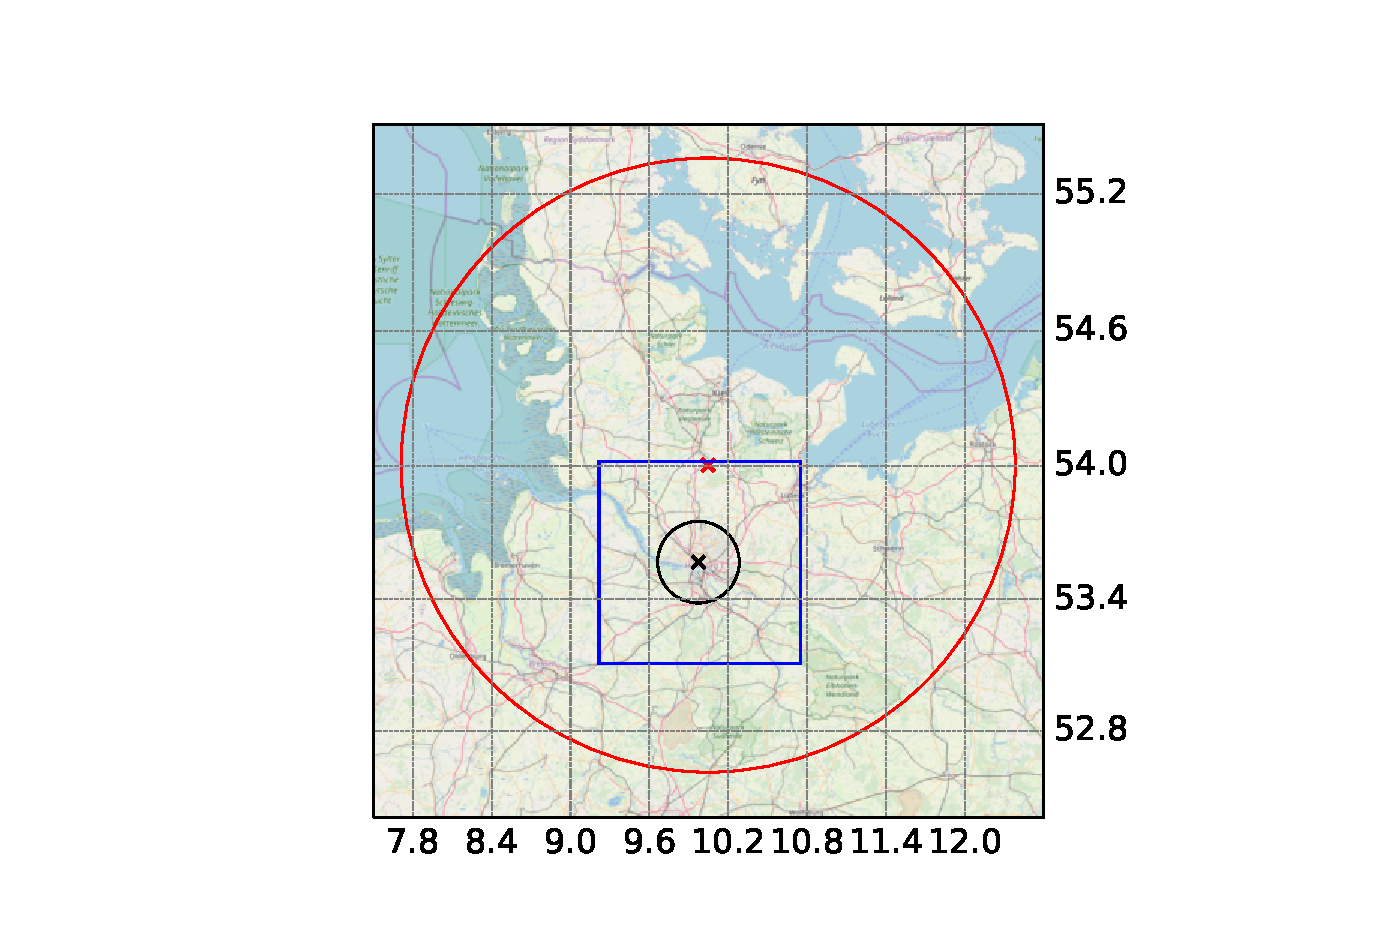
\includegraphics[width=\textwidth,trim={11cm 0 11cm 0}, clip]{radarOverview.eps}
	\caption{Radaroverview. Red: Boostedt precip sweep, Black: Pattern precip sweep, Blue: Nesting area from boostedt radar sweep}
	\label{fig:radarOverview}
\end{figure}
\chapter{Methodology}
\section{Prognosis Model}
\subsection{Setting of Parameters}
\subsection{Gridding and Coordinate Transformation}
Both the DWD and PATTERN radar data are initially in a polar grid around their respective radar stations. For simplicity, nesting/comparability between both radars and to regard the curvature of the earth, the polar data is transformed and gridded to a Cartesian grid. 

This is done by using the Transverse Mercator projection transforming the polar grid coordinates to a Cartesian grid. The Transverse Mercator projection divides the Earth into 60 zones with  6° longitude in width. This reduces the distortion due to the curvature of the earth. Hamburg and its surrounding area lies in the EPSG zone 32632. 

\begin{figure}
	\centering
	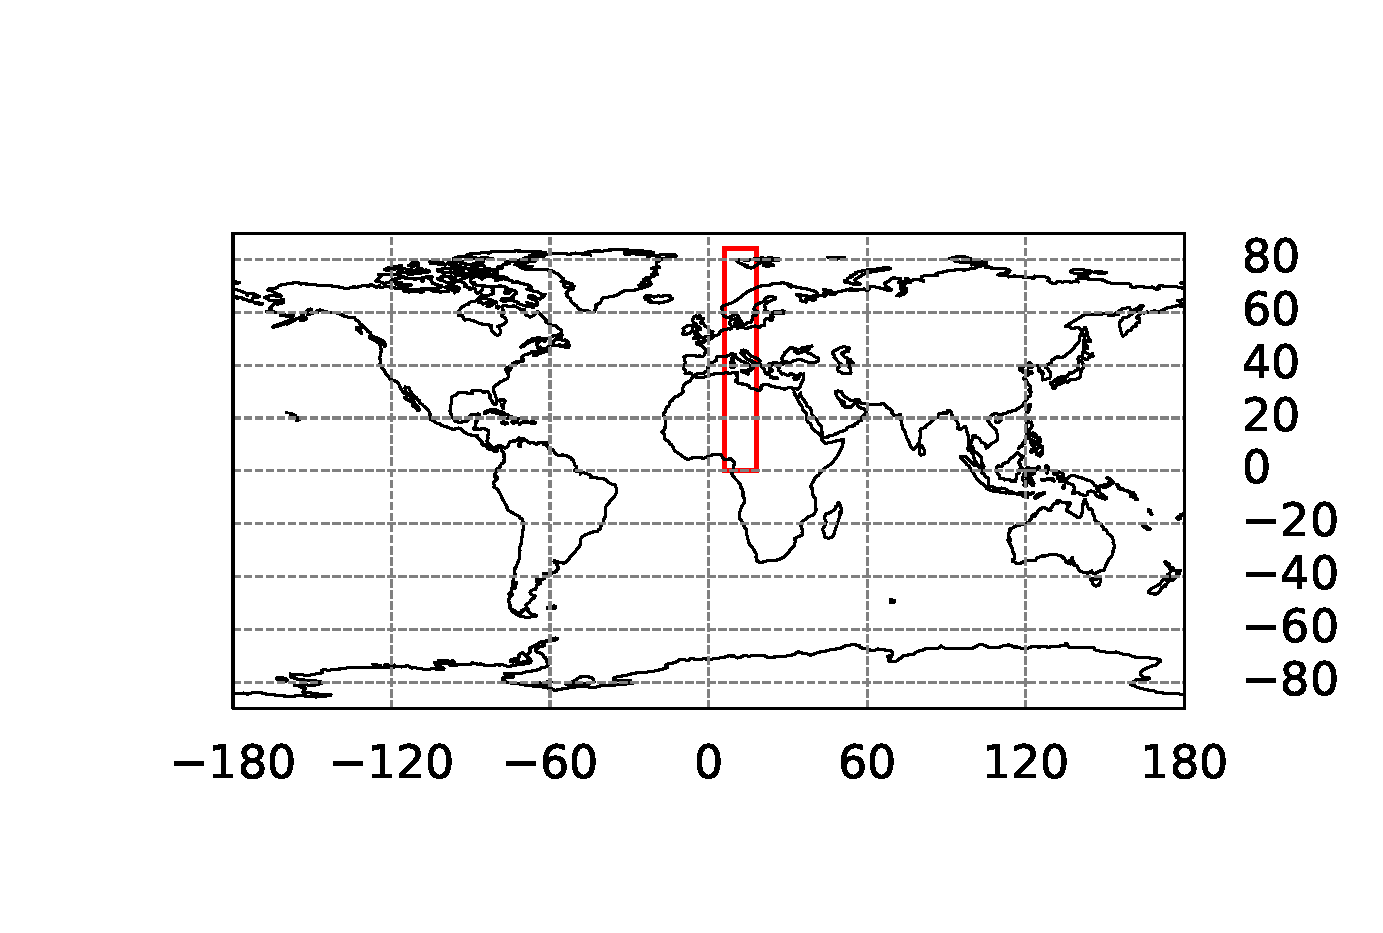
\includegraphics[width=\textwidth]{EPSG2.eps}
	\caption{EPSG Overview}
\end{figure}

Displacing the point of origin in the coordinate system from the point of the radar to the EPSG zone 32632.
\begin{equation}
	\begin{array}{lcl}
		x = r \cdot \cos(azi)\\
		y = r \cdot \sin(azi)
	\end{array}	
\end{equation}

\begin{equation}
	Z  = 10 \cdot \log _{10}(z)
\end{equation}

\begin{equation}
	z = aR^{b}
\end{equation}

\begin{equation}
	R = \frac{Z}{a}^{\frac{1}{b}}
\end{equation}
a and b are empirically-derived parameters. DWD and PATTERN use following values for the z-r relation for different radar reflectivities:

\begin{equation}
	\begin{array}{lcl}
		Z \le 36.5 \text{dBZ}: & a = 320, b = 1.4 \\
		36.5 \text{dBZ} < Z \le 44.0 \text{dBZ}: & a  = 200, b = 1.6 \\
		Z > 44.0 \text{dBZ}: & a = 77, b = 1.9
	\end{array}
\end{equation}

\subsection{Interpolation Methods}
\subsubsection{Barycentric Interpolation}
To transform the data from a polar grid to a Cartesian grid a Barycentric interpolation is applied to the radar data. The Barycentric interpolation is implemented following \cite{bary}. 

For the two dimensional barycentric interpolation the first step is to arrange the initial grid, here a polar grid around the radar site, into triangles. A possible way to do this is using the Delaunay Triangulation after \cite{delaunay}. This triangulation triangulates a set of points \textbf{P} so that no point in \textbf{P} is inside of the circumcircle of any triangle. Now the surrounding triangle is known for each point of the Cartesian grid.

In comparison to coordinate systems like Cartesian or polar coordinate systems where points are offsets to a origin, barycentric coordinates describe the position of points relative to a simplex (e.g. a line, a triangle or a tetrahedron) (\citealp{bary} and \citealp{baryBerrut}). In this case barycentric coordinates are used to compare positions of points to triangles. For triangles barycentric coordinates can be understood as area coordinates. The equations to calculate the barycentric coordinates $d,e,g$ of the point $P$ in the triangle $A,B,C$ are ratios of their respective triangles and the total triangle(Fig. \ref{fig:bary}). For example the coordinate $g$ is calculated by dividing the area of the triangle $CAP$ by the area of the triangle $ABC$ (\ref{eq:barycor}).

Now to get the value $f(x_p,y_p)$, the values of the points $A,B,C$ are weighted by their respective coordinate $d,e,g$ and summed up (eq. \ref{eq:baryeq}).
\begin{figure}
	\centering
	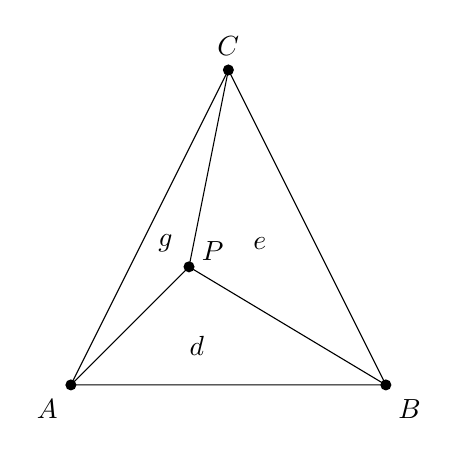
\begin{tikzpicture}
	
	\draw (0,0) -- (2,4) -- (4,0) -- (0,0);
	\fill (1.5,1.5) circle[radius=2pt];
	\fill (0,0) circle[radius=2pt];
	\fill (2,4) circle[radius=2pt];	
	\fill (4,0) circle[radius=2pt];	
	\draw (0,0) -- (1.5,1.5);
	\draw (2,4) -- (1.5,1.5);
	\draw (4,0) -- (1.5,1.5);
	
%	\draw (-0.3,-0.3) node {$(x_1,y_1)$};
%	\draw (4.3,-0.3) node {$(x_2,y_2)$};
%	\draw (2,4.3) node {$(x_3,y_3)$};
%	\draw (1.6,1) node {$(x,y)$};
	\draw (-0.3,-0.3) node {$A$};
	\draw (4.3,-0.3) node {$B$};
	\draw (2,4.3) node {$C$};
	\draw (1.8,1.7) node {$P$};
	
	\draw (1.6,0.5) node {$d$};
	\draw (2.4,1.8) node {$e$};
	\draw (1.2,1.8) node {$g$};
				
	\end{tikzpicture}
	\caption{Barycentric interpolation in a triangle}
	\label{fig:bary}
\end{figure}


\begin{equation}
	\begin{aligned}
		d = \dfrac{\Delta ABP}{\Delta ABC}\\
		e = \dfrac{\Delta BCP}{\Delta ABC}\\
		g = \dfrac{\Delta CAP}{\Delta ABC}
	\end{aligned}
	\label{eq:barycor}
\end{equation}

\begin{equation}
f(x_P,y_P) = d\,f(x_A,y_A)+e\,f(x_B,y_B)+g\,f(x_C,y_C)
\label{eq:baryeq}
\end{equation}

\subsubsection{Bilinear Interpolation}
Following a similiar approach as \cite{bilinear} the bilinear interpolation is implemented as the equation \ref{eq:bilinear}. The bilinear interpolation is used for datapoints which lie inside of a square Cartesian grid. This is depicted in Fig. \ref{fig:bilinear}. The point $(x,y)$ is surrounded by the points $(x_1,y_1),(x_2,y_1),(x_2,y_2),(x_1,y_2)$. Now to calculate the value $f(x,y)$, the values of the surrounding points $f(x_1,y_1),f(x_2,y_1),f(x_2,y_2),f(x_1,y_2)$ are weighted with their respective opposite areas $m,n,o,p $ and are summed up. 


\begin{figure}[H]
	\centering
	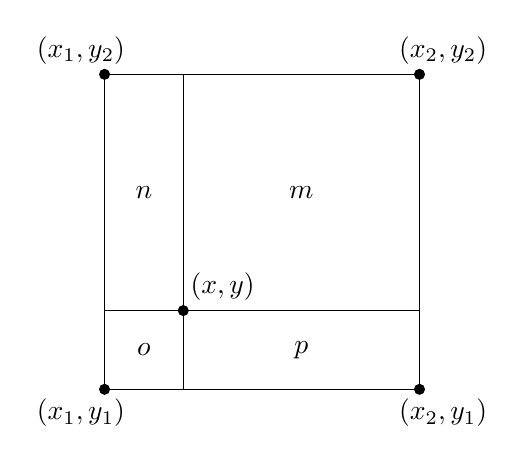
\begin{tikzpicture}
	\draw (0,0) rectangle (4,4);
	\draw (0,0) rectangle (1,1);
	\draw (1,1) rectangle (4,4);
	\fill (0,0) circle[radius=2pt];
	\fill (0,4) circle[radius=2pt];
	\fill (4,0) circle[radius=2pt];
	\fill (4,4) circle[radius=2pt];
	\fill (1,1) circle[radius=2pt];
	\draw (-0.3,-0.3) node {$(x_1,y_1)$};
	\draw (-0.3,4.3) node {$(x_1,y_2)$};
	\draw (4.3,-0.3) node {$(x_2,y_1)$};
	\draw (4.3,4.3) node {$(x_2,y_2)$};
	\draw (1.5,1.3) node {$(x,y)$};
	\draw (2.5,2.5) node {$m$};
	\draw (0.5,2.5) node {$n$};
	\draw (0.5,0.5) node {$o$};
	\draw (2.5,0.5) node {$p$};
	\end{tikzpicture}
	\caption{Bilinear Interpolation}
	\label{fig:bilinear}	
\end{figure}

\begin{equation}
	f(x,y) = m\,f(x_1,y_1)+n\,f(x_2,y_1)+o\,f(x_2,y_2)+p\,f(x_1,y_2)
	\label{eq:bilinear}
\end{equation}
\subsection{Displacement Detection}
In this thesis a combination of a cell and field-based algorithm is used.

In order to make a prognosis on the movement of precipitation fields a displacement vector is needed and several approximations are necessary. 

To find displacement vectors the following procedure is applied to the precipitation fields of the PATTERN and DWD radar.
\begin{enumerate}
	\item Detection of suitable patches in the precipitation field for tracking (Fig. \ref{fig:maximaOverview}).
	\item Tracking of the patches over the evolution of several time steps.
	\item If patches move out of the frame or become undesirable to be tracked new patches are searched in the actual time step.
	\item Tracks of each patch are evaluated.
\end{enumerate}
Least square correlation
\begin{figure}[H]
	\centering
	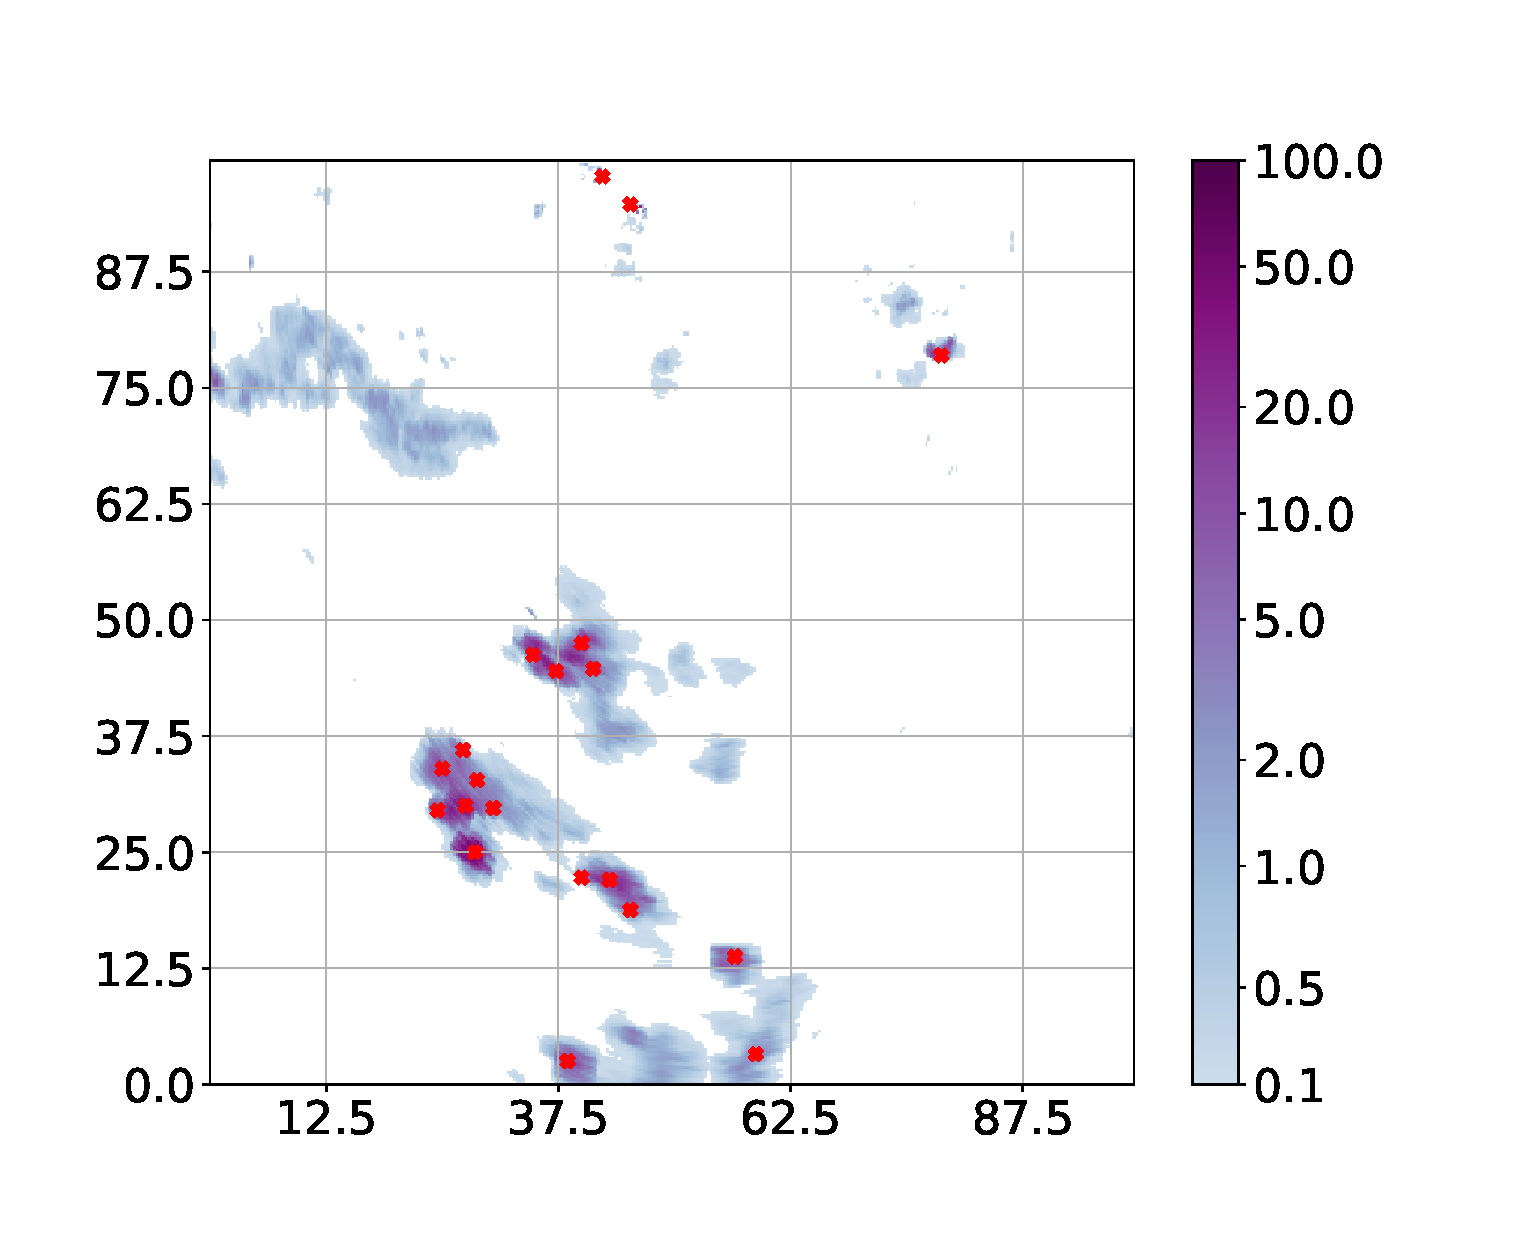
\includegraphics[width=\textwidth]{maximaOverview.eps}
	\caption{Boostedt radar, with the maxima marked with 'x'}
	\label{fig:maximaOverview}
\end{figure}
\begin{figure}[h]
	\centering
	\begin{minipage}{0.45\textwidth}
		\includegraphics[width=\textwidth,trim={15mm 0 15mm 0},clip]{Displacement_t0.png}
		\caption{Sector of the boostedt radar at timestep t}
		\label{fig:displacement_t0}
	\end{minipage}\hfill
	\begin{minipage}{0.45\textwidth}
		\includegraphics[width=\textwidth,trim={15mm 0 15mm 0},clip]{Displacement_t1.png}
		\caption{Sector of the boostedt radar at timestep t+1}
		\label{fig:displacment_t1}
	\end{minipage}

\end{figure}

\begin{figure}[ht]
	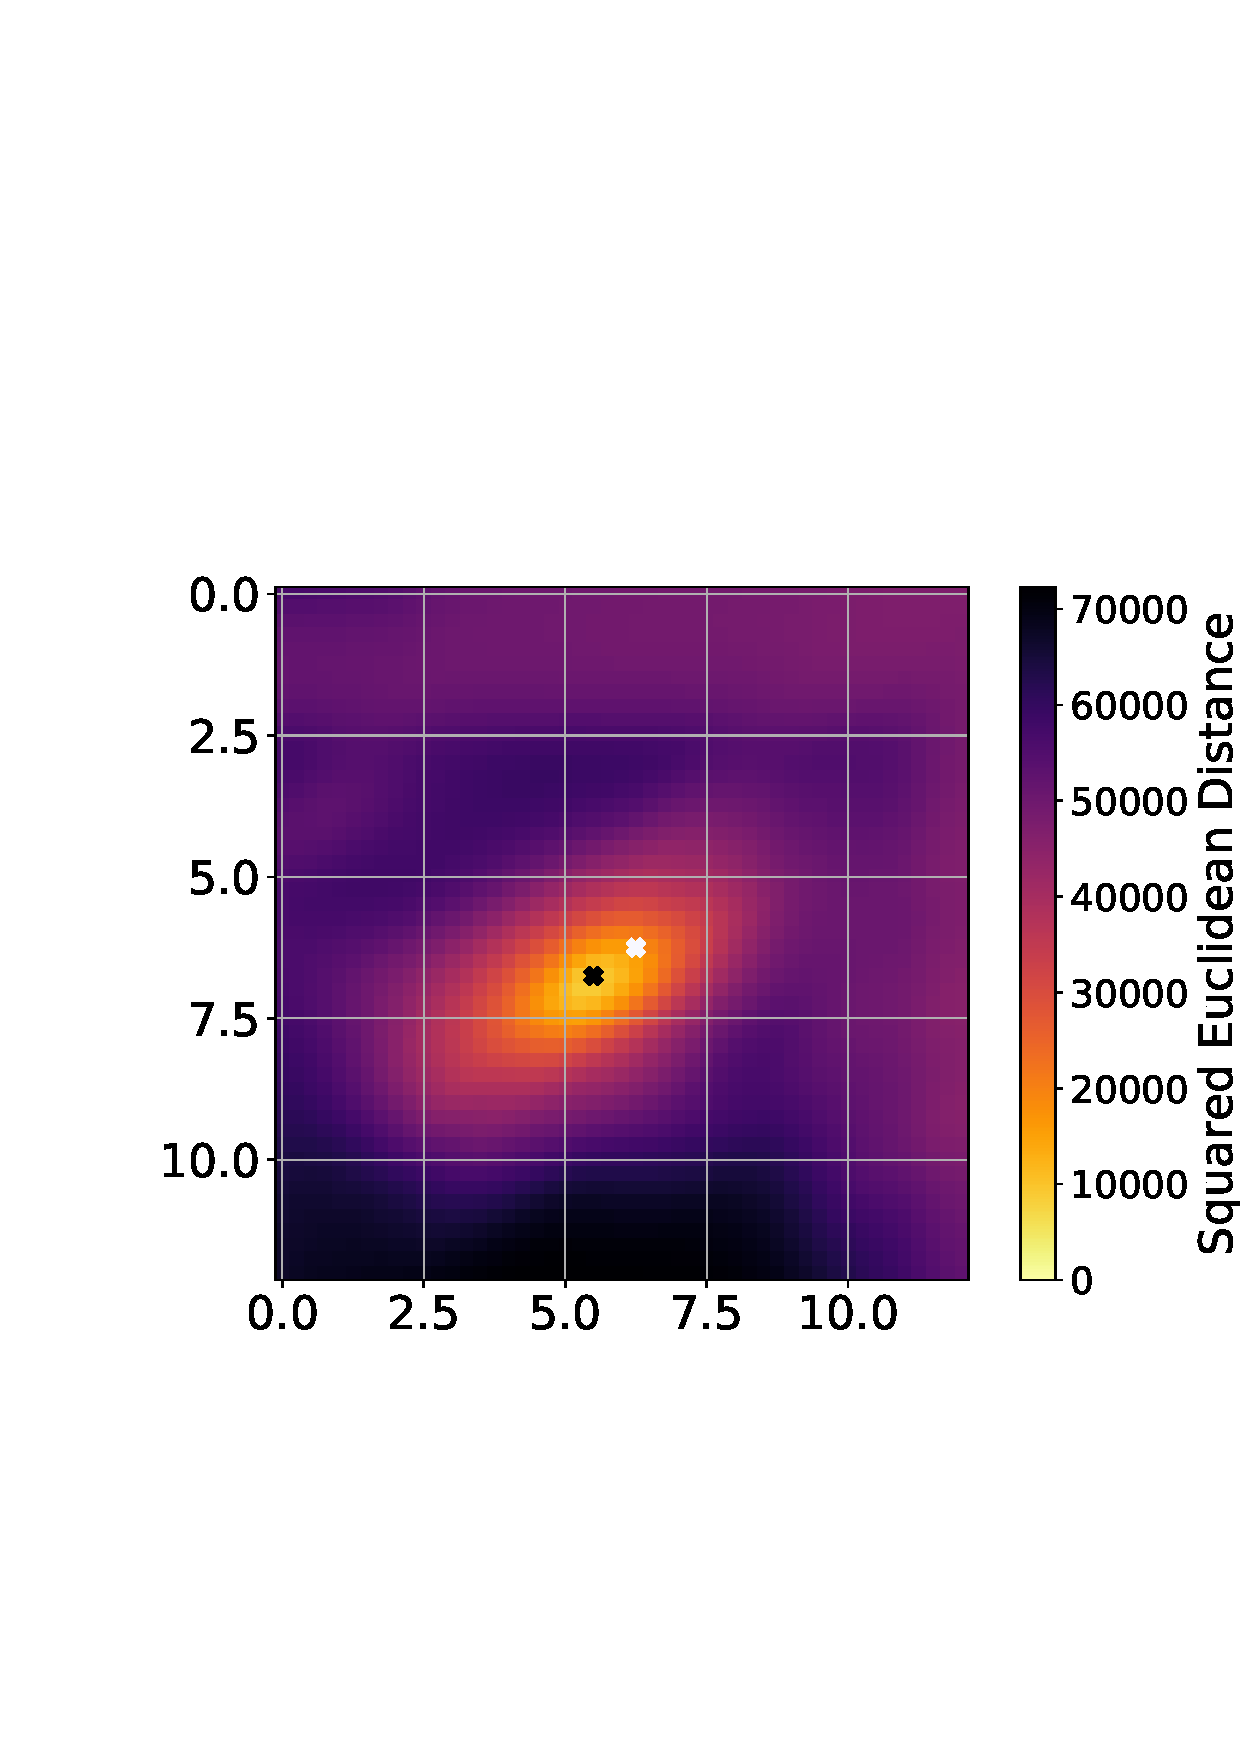
\includegraphics[width=\textwidth,trim={15mm 0 15mm 0},clip]{Correlation_Matrix.png}
	\caption{Correlation Matrix between the red area from \ref{fig:displacement_t0} and the total area of \ref{fig:displacment_t1}}
	\label{fig:corr_matrix}
\end{figure}
%http://www.cs.umd.edu/~djacobs/CMSC426/Convolution.pdf
\begin{equation}
	d^2_{q,p}(u,v) = \sum_{x,y}^{}\big[q(x,y)-p(x-u,y-v)\big]^2
\end{equation}
\subsection{Bivariate Normal Densities}
With $\sigma_1^2$ as $\sigma_{11}$ and $\sigma_1 \cdot\sigma_2$ as $\sigma_{12}$
\begin{equation}
	\rho = \dfrac{\sigma_{12}}{\sigma_1\sigma_2}
\end{equation}
\begin{equation}
	\begin{multlined}
		p_{x1x2}(x_1,x_2)=\dfrac{1}{2\pi\sigma_1\sigma_2\sqrt{1-\rho^2}} \times \\ e^{-\dfrac{1}{2(1-\rho^2)}\bigg[\bigg(\dfrac{x_1-\mu_1}{\sigma_1}\bigg)^2-2\rho\bigg(\dfrac{x_1-\mu_1}{\sigma_1}\bigg)\bigg(\dfrac{x_2-\mu_2}{\sigma_2}\bigg)+\bigg(\dfrac{x_2-\mu_2}{\sigma_2}\bigg)^2\bigg]}
	\end{multlined}
\end{equation}


\subsection{Importance Sampling}
	\begin{figure}[H]
	\centering
	\begin{tikzpicture}
    \begin{axis}[
	axis x line=center,
	axis y line=center,
	xtick={0,1,...,4},
	ytick={0,1,...,4},
	grid=major,
	xmin=0,
	ymin=0,
	xmax=4,
	ymax=4
    ]
	\fill (3,3) circle[radius=2pt];

	\draw (3.32,3.3) node {$f(x,y)$};

	\foreach \x in {0, ..., 24} {%A,mu,sigma,x
		\pgfmathsetmacro{\xcoor}{rand}% x-coordinate
		\edef\temp{
			%\noexpand\coordinate (A) at ({gauss(1,0,1,\xcoor)},{gauss(1,0,1,\xcoor)});
			\noexpand\coordinate (A) at ({invgauss(rnd,rnd)/4+1},{invgauss(rnd,rnd)/4+1});
			\noexpand\draw (A) -- (3,3);	
			\noexpand\fill (A) circle[radius=1pt];
		}
	\temp
	}
	%\draw (1.5,0.5) --(3,3);
	%\fill (1.5,0.5) circle[radius=2pt];
	\draw (1.5,0.5) node {$f(x_s,y_s)$};

    \end{axis}
	\end{tikzpicture}
	\caption{Normal Distribution with $\mu$ = 1 and $\sigma$ = 1/4}
	\label{fig:importancesampling}
\end{figure}


\begin{equation}
	f_{t+1}(x,y) = \frac{1}{N}\sum_{s=0}^{N} f_{t}(x_s,y_s)
\end{equation}
\section{Evaluation Methods}
\subsection{Point to Point Evaluation}
A rain threshold is set. Rainrates above that value e.g. 0.5 are considered to be rain, thus represented with a 1. Rainrates below that value are no rain, thus represented with a 0. Applying this threshold for the total rainfield creates a matrix of 0s and 1s. Now rainfields of the forecast and the reference values are compared.
\begin{enumerate}
	\item Hit(\textbf{H}): Both forecast and reference points show rain
	\item Miss(\textbf{M}): Reference point shows rain, forecast shows no rain
	\item False Alert(\textbf{FA}): Forecast shows rain, reference shows no rain
	\item Correct Rejection(\textbf{CR}): Both forecast and reference points show no rain
\end{enumerate}
From the ratios of these 4 cases it is possible to derive several skill scores:
\begin{equation}
\begin{array}{lcl}
	PC = \dfrac{H+CR}{H+M+FA+CR}\\
	POD = \dfrac{H}{H+M}\\
	FAR = \dfrac{FA}{FA+H}\\
	CSI = \dfrac{H}{H+M+FA}\\
	ORSS = \dfrac{H\cdot CR-FA\cdot M}{H\cdot CR+FA\cdot M}
\end{array}
\end{equation}
\chapter{Results and Discussion}
\chapter{Conclusion and Outlook}
\chapter{Acknowledgement}
\bibliography{References}
\chapter{Eidesstattliche Versicherung}
Ich versichere an Eides statt, dass ich diese Arbeit selbstständig verfasst und keine anderen als die angegebenen Hilfsmittel benutzt habe. Insbesondere habe ich keine im Literaturverzeichnis nicht genannten Internet-Quellen benutzt. Diese Arbeit habe ich vorher nicht in einem anderen Prüfungsverfahren eingereicht und die eingereichte schriftliche Fassung entspricht der Fassung auf dem elektronischen Speichermedium. Ich stimme einer Veröffentlichung dieser Arbeit zu.
\\
\\
\\
\\
\\
Simon Michel\\
Hamburg, \today
\end{document}

